\documentclass[12pt]{article}


%%%%%%%%%%%%%%%%%%%%%%%%%%%%%%%%%%%%%%%%%%%%%%%%%%%%%%%%%%%%%%%%%%%%%%%%%%%%%%%%%%%%%%
%%%%%%%%%%%%%%%%%%% YOU PROBABLY DON"T NEED TO CHANGE ANYTHING HERE %%%%%%%%%%%%%%%%%%%
\usepackage[numbers,sort]{natbib}
\usepackage{amsfonts, amsmath} 
\usepackage{graphicx}
\usepackage{libertine} 
\usepackage{fullpage}
\usepackage{hyperref}
\usepackage{booktabs}   % table rules
\usepackage{xcolor}
\hypersetup{
    colorlinks = true,
    linkcolor = blue,
    urlcolor  = blue,
    citecolor = blue,
    anchorcolor = blue}
\urlstyle{same}
% placeholders: shown in red until filled; search for \tbc before submitting
\newcommand{\tbc}[1]{\textcolor{red}{\textbf{[TBC: #1]}}}

%
% ===== DOCUMENT STARTS HERE =======
%
\begin{document}

\title{Model Size and Data Repetition under a Fixed Compute Budget}
\date{\today}
\maketitle

{\bf Group Composition:}
\begin{enumerate}
\item {Jia Sijia, A0282953U, e1157081@u.nus.edu}
\item {Lim Yu Ki, A0281618Y, e1155746@u.nus.edu}
\item {Yap Xin Yu, A0281772X, e1155900@u.nus.edu}
\end{enumerate}

{\bf Github Repository:} \url{https://github.com/phoebeyap04/dsa4212-small-llm}

\section{Introduction}

Training a language model always happens under a compute budget, and the same budget can be spent in different ways: on a larger model that learns more per token but processes fewer tokens, or on a smaller, faster model that sees more text. \citet{hoffmann2022training} estimated that, under their compute-optimal setup for large models, the best balance is roughly 20 training tokens per parameter. Unique data is also limited in practice, so a model may have to reread the same text; \citet{muennighoff2023scaling} found that repeated data is almost as valuable as fresh data for a few passes and loses value after that.
 
We study both trade-offs at a small scale, where they are cheap to test: \emph{within one hour of training on a single GPU, does a smaller model that processes more text outperform a larger one, and does the answer change when unique data is limited, so that models must repeat it?}
 
We train decoder-only Transformers of three sizes (3.1M, 10.6M and 25.2M non-embedding parameters) from scratch on TinyStories \citep{eldan2023tinystories}. Each is trained on either a small pool of 10,000 stories or a large pool of 1,000,000 stories, with two random seeds (12 runs in total). We compare the models on a held-out test set, both at the end of training and at the point of lowest validation loss. On the large pool, the largest model achieves the lowest test loss, although its gain over the medium model is small. On the small pool, all three sizes overfit after 7--9 passes, and keeping the checkpoint with the lowest validation loss reduces test loss by more than 2.3 nats per token at every size, far more than the choice of model size.

\section{Setup}

\paragraph{Compute budget.} We limit each run to \textbf{3,600 seconds of training time on one NVIDIA T4 GPU} (Google Colab or Kaggle). We time only the optimisation steps, and exclude evaluation, checkpointing, data preparation, tokeniser training and final testing. About 10 seconds of one-off model compilation falls inside the first timed steps (under 0.3\% of the budget). If a run is resumed, its clock continues where it stopped. We do not report the short preliminary runs we used to test the pipeline. Our budget therefore fixes training time on a given GPU rather than the number of operations: larger models use the GPU more efficiently and complete more operations within the same hour (Section~\ref{sec:discussion}).
 
\paragraph{Initialisation.} We train all models from random initialisation using the nanoGPT implementation \citep{karpathy2022nanogpt}. We use no pretrained weights, embeddings or components, and we trained the tokeniser ourselves on training data only. Every run starts at a loss between 9.00 and 9.10 nats, matching uniform guessing over the 8,000-token vocabulary ($\ln 8000 \approx 8.99$).
 
\paragraph{Evaluation.} We report final results on a held-out test set of 7,350 TinyStories stories (1.55M tokens), which is held out from training and checkpoint selection and evaluated only after both are complete. We use a separate validation set during training and to select the best checkpoint. The metric is token-weighted cross-entropy, comparable across runs because all models share one tokeniser. It measures how well a model predicts unseen text, not whether its stories are coherent (Section~\ref{sec:limitations}).

% ---------- 3: Yuki ----------
\section{Data}
\label{sec:data}

\paragraph{Datasets and Splits.} We utilise the \textbf{TinyStories dataset} \citep{eldan2023tinystories}, a synthetic corpus of short narratives restricted to an early-childhood vocabulary, which allows small language models to acquire basic syntactic competence within a strict compute budget. 
We used the official training split as the source for our training pools. To form our evaluation sets, we divided the official validation split by whole stories to create disjoint validation and held-out test sets.

\paragraph{Preprocessing and Deduplication.} To mitigate data leakage and memorisation artefacts, we identified exact duplicate stories by comparing them after stripping surrounding whitespace and converting to lowercase; this normalisation was used only for comparison, and the stories themselves were kept unchanged.
We then removed over 320,000 exact duplicates from the training data. However, we do acknowledge the \textbf{limitation} that it may not capture all near-duplicate semantic variations.

\paragraph{Nested Pools.} We constructed two nested training pools (Figure \ref{fig:pipeline}). After, we shuffled the deduplicated training stories once using a fixed random seed to ensure pool membership remained immutable across all training runs and seeds. The small pool consists of an initial subset of 10,000 stories, while the large pool consists of 1,000,000 stories. Because the large pool is a superset of the small pool, the design shows how additional unique training data affects performance under a fixed training-time budget, with smaller pools leading to more repeated exposure \cite{muennighoff2023scaling}.

\begin{figure}[h]
\centering
\begin{verbatim}
TinyStories Dataset
 | Official Train Split 
 |      Deduplication (320,470 exact duplicates removed)
 |          Shuffled (Fixed Random Seed)
 |              Small Pool (First 10,000 stories) 
 |              Large Pool (1M stories; strictly includes Small Pool)
 |
 | Official Validation Split
     | Halved, then deduplicated (against training and each other)
         | Validation Set (8,039 stories)
         | Test Set (7,350 stories; strictly held-out)
\end{verbatim}
\caption{Data preprocessing and splitting pipeline.}
\label{fig:pipeline}
\end{figure}

\paragraph{Shared Tokeniser.} We trained a Byte-level Byte-Pair Encoding (BPE) tokeniser capped at an 8,000-token vocabulary. This vocabulary size prevents the embedding matrix from disproportionately consuming the parameter budget of our smaller model configurations. The tokeniser was trained exclusively on the large training pool and was subsequently frozen. Sharing this single frozen tokeniser across the six model configurations ensures that our token-weighted cross-entropy measurements remain directly comparable.

\begin{table}[h]
\centering
\caption{Dataset statistics after deduplication and tokenisation.}
\label{tab:dataset_stats}
\begin{tabular}{lrrl}
\toprule
\textbf{Split} & \textbf{Story Count} & \textbf{Token Count} & \textbf{Experimental Function} \\
\midrule
Train (Small) & 10,000 & 2,203,244 & High-repetition exposure baseline \\
Train (Large) & 1,000,000 & 219,406,952 & Low-repetition exposure baseline \\
Validation & 8,039 & 1,601,531 & Periodic evaluation during training \\
Test (Held-out) & 7,350 & 1,551,129 & Final checkpoint benchmarking \\
\bottomrule
\end{tabular}
\end{table}

\paragraph{Deterministic Evaluation.} To eliminate the sampling noise of nanoGPT's randomly sampled evaluation batches \citep{karpathy2022nanogpt}, we evaluate final results with a separate deterministic script. During evaluation, models process the validation and test sets in sequential and non-overlapping blocks. Our primary metric, token-weighted cross-entropy, measures how well each next token is predicted on these fixed blocks.
However, we do note that this metric evaluates predictive probability distributions and penalises vocabulary uncertainty hence it does not evaluate semantic story coherence, which requires separate inspections \citep{eldan2023tinystories}.

% ---------- 4: Pb ----------
\section{Method}
\label{sec:method}

We use the same code and settings for every run and change only the model size and the training pool. We use nanoGPT, which we modified to enforce a training-time budget, schedule the learning rate by time, log tokens seen and epochs, keep the lowest-validation-loss checkpoint, and resume without resetting the clock.
 
\paragraph{Models and throughput.} We scale depth and width together (Table~\ref{tab:models}) and report non-embedding parameters as model size (excluding the token and position embedding tables; the output layer shares the token embedding's weights), following \citet{kaplan2020scaling}, since the embedding table accounts for 40\% of the small model's parameters. Larger models process fewer tokens per hour, which is the trade-off under study. The large model has $8.0\times$ the parameters of the small one but is only $4.8\times$ slower, as small models do not use the GPU fully. Dividing tokens seen by non-embedding parameters gives tokens per parameter: 359 for the small model, 45 for the medium and 9.4 for the large. The roughly 20 that \citet{hoffmann2022training} found compute-optimal therefore lies between our medium and large models.
 
\begin{table}[ht]
\centering
\small
\caption{Model sizes and throughput in one hour. Tokens/s and tokens seen are averaged over each size's four runs; passes over each pool are averaged over the two runs trained on that pool.}
\label{tab:models}
\begin{tabular}{lrrrrrrrr}
\toprule
 & & & Non-emb. & Total & & Tokens & \multicolumn{2}{c}{Passes over pool} \\
Model & Layers & Width & params & params & Tokens/s & seen & small & large \\
\midrule
Small  & 4 & 256 & 3.15M  & 5.26M  & 313,000 & 1,129M & 517 & 5.1 \\
Medium & 6 & 384 & 10.62M & 13.79M & 132,000 & 474M   & 221 & 2.1 \\
Large  & 8 & 512 & 25.17M & 29.40M & 66,000  & 237M   & 116 & 1.0 \\
\bottomrule
\end{tabular}
\end{table}
 
\paragraph{Training settings.} In every run we use a context length of 256 and a batch size of 32 (8,192 tokens per step); AdamW ($\beta_2=0.99$, weight decay 0.1, gradient clipping 1.0); a learning rate warmed up over 200 steps to $10^{-3}$ and cosine-decayed to $10^{-4}$; no dropout; float16 mixed precision; and one attention head per 64 dimensions of width. Every 500 steps, we measure the loss on fixed train and validation subsets.
 
\paragraph{Enforcing the budget.} A fixed step count would give the models unequal budgets, since steps take longer for larger models. Instead, we measure the duration of each optimisation step, waiting for the GPU to finish so that the clock reflects actual computation, and stop training once the total reaches 3,600 seconds; the learning rate decays by the fraction of the budget used, so every model completes its schedule as its hour ends. Eleven runs ended at 3,600.0--3,600.1\,s and one, accidentally resumed for a single extra step, at 3,603.8\,s.

 \paragraph{Checkpoints.} Preliminary runs showed validation loss on the small pool reaching a minimum early and then rising as the model memorises the stories. We therefore keep the \emph{final} checkpoint and the \emph{best} (lowest validation loss) checkpoint of each run, and evaluate both on the test set. The best checkpoint is chosen from the periodic validation estimates on a fixed subset of about 820,000 validation tokens rather than a full validation pass; selection uses validation data only, so the test set stays untouched until final evaluation. For example, the large model on the small pool reached its lowest validation loss of 2.46 after 7.4 passes, but ended at 4.78.
 
\paragraph{Platforms.} We ran the experiments on Google Colab and, once its free GPU allowance ran out, on Kaggle, using the same GPU model (NVIDIA T4), code and data on both. Throughput of the same model varied between sessions by up to a third (large model: 58,000--77,000 tokens/s), so we report the number of tokens seen for every run.

\section{Results}
\label{sec:results}

\paragraph{Validation loss during training.}
On the 10,000-story pool, all six runs reached their lowest recorded
validation loss after 7.4--9.3 effective passes over the training pool
(Figure~\ref{fig:validation-loss}). Validation loss rose from minima
of 2.44--2.48 to 4.78--6.14 by the end of the hour, even though final
training loss was below 0.19 for every run. This pattern is consistent
with overfitting under repeated exposure to the small pool. On the
1,000,000-story pool, validation loss continued to improve towards the
end of training for all three model sizes and both seeds.

\begin{figure}[htbp]
    \centering
    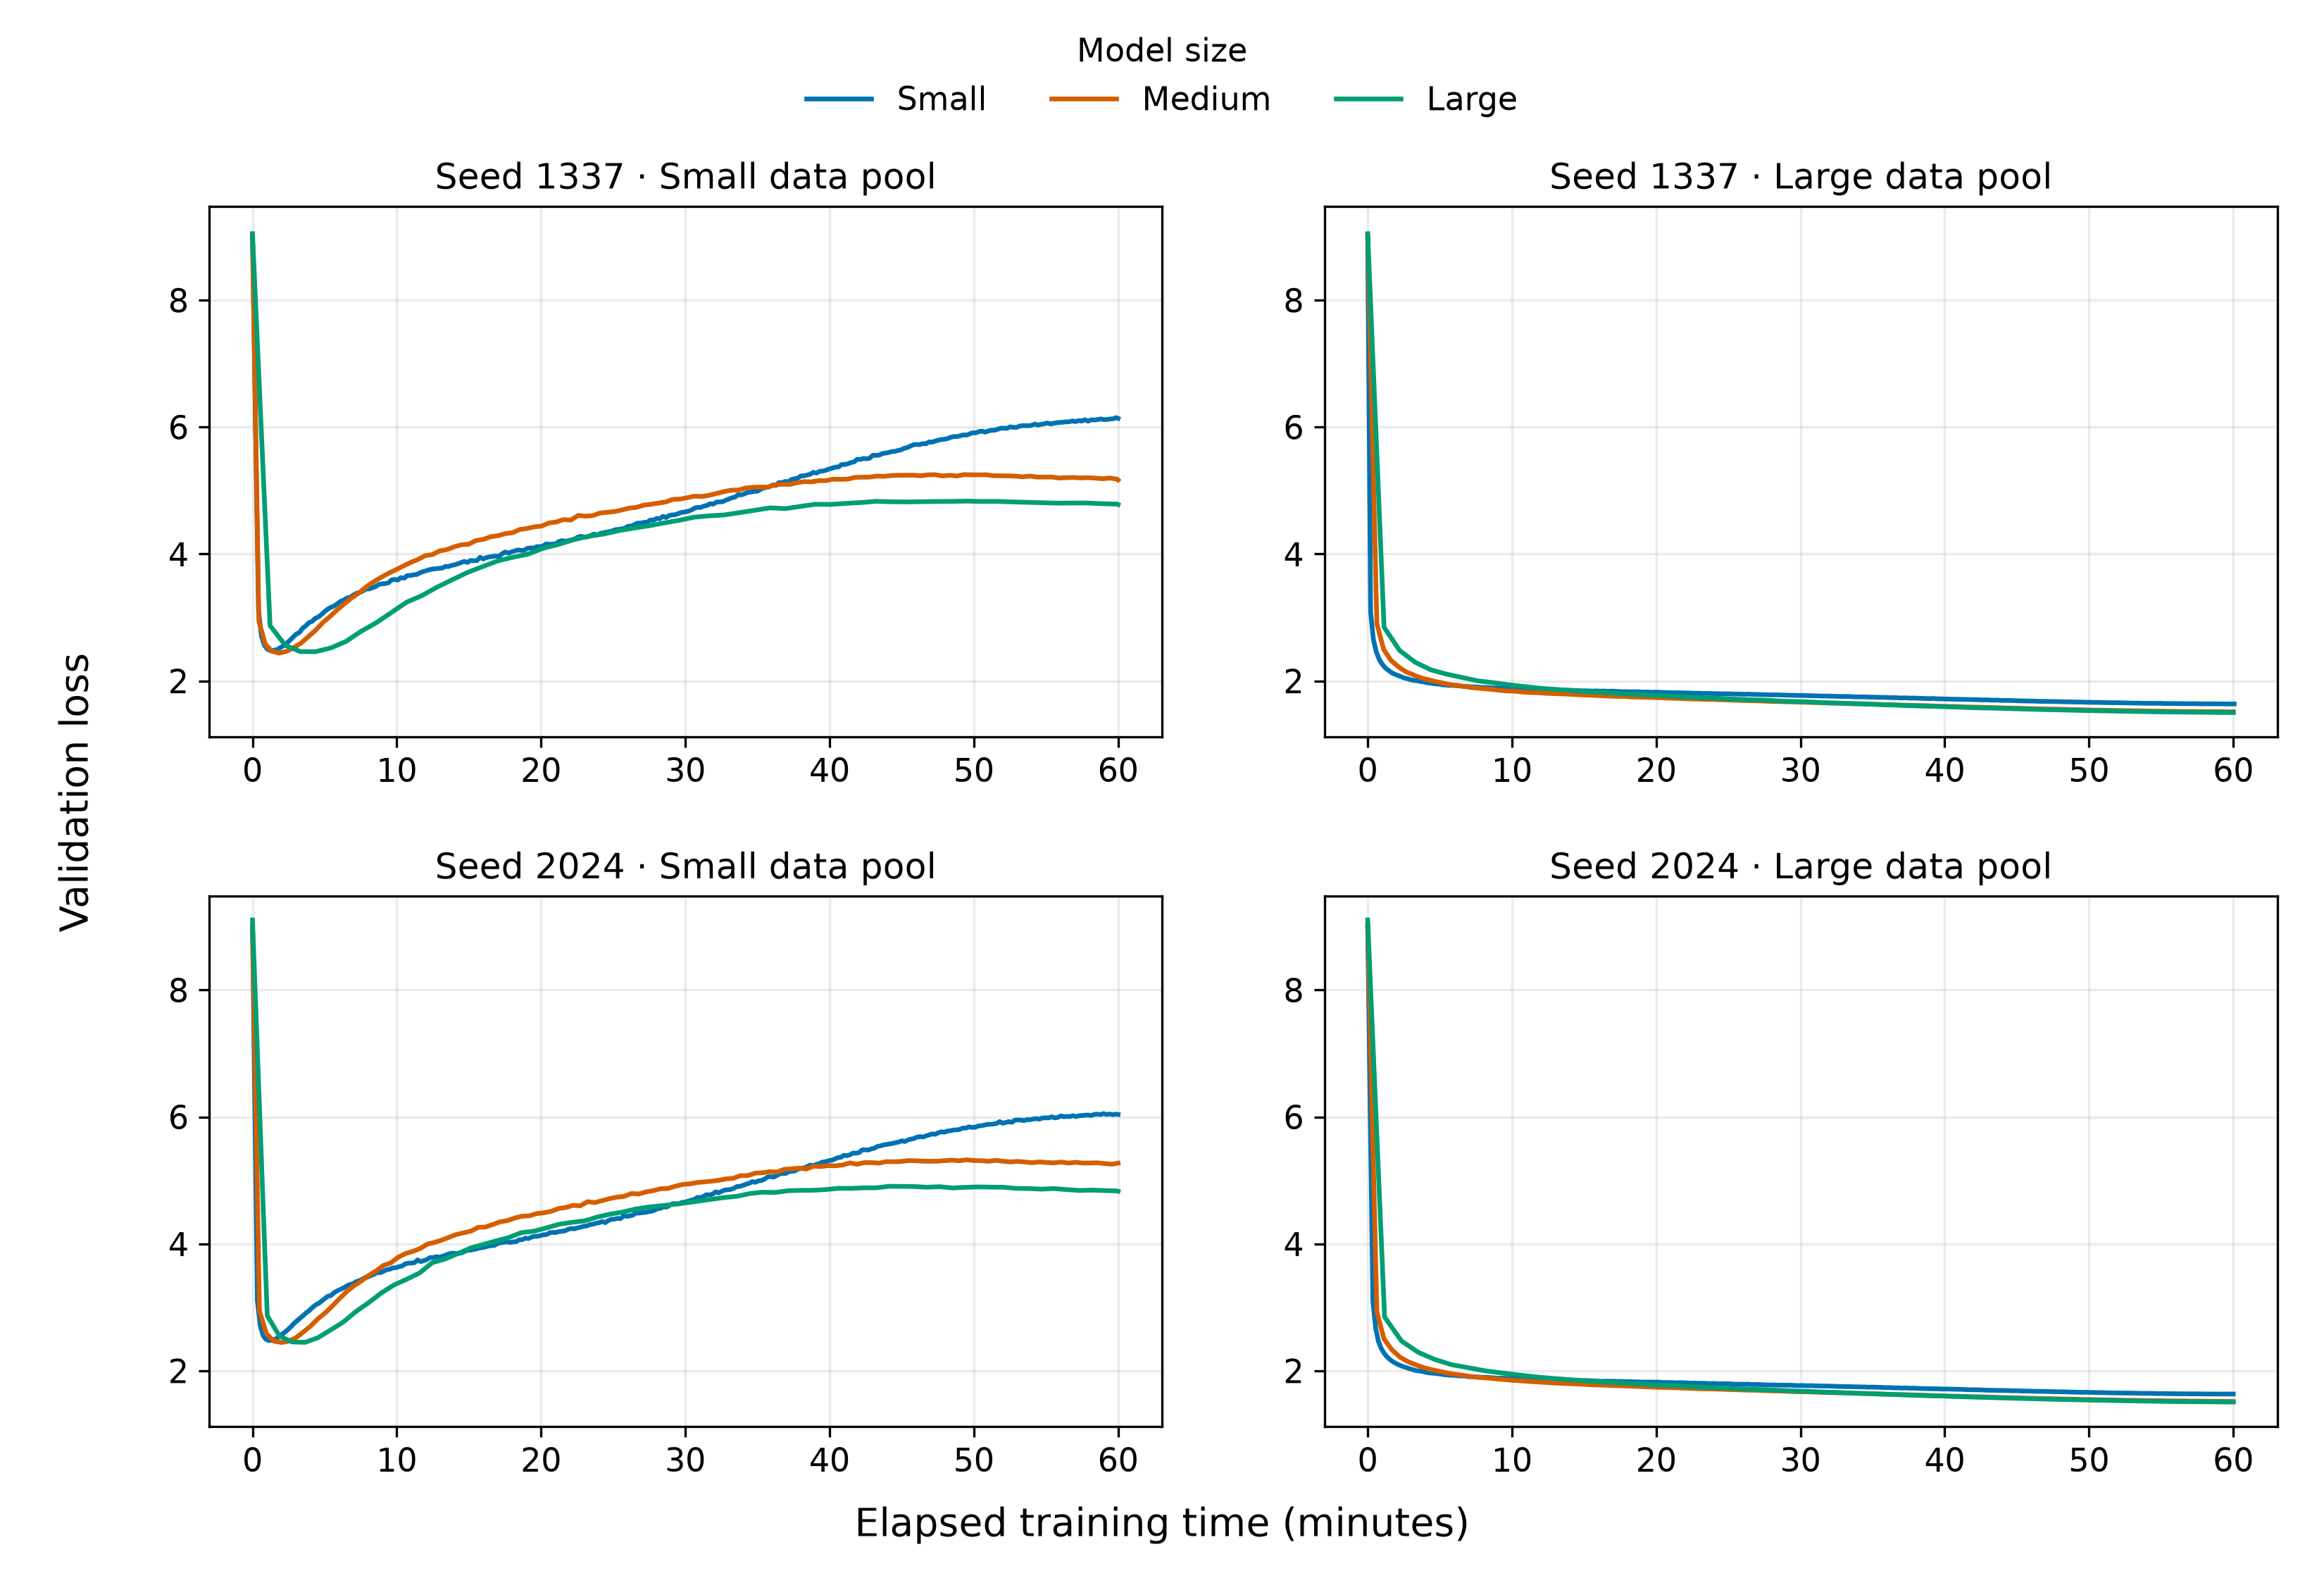
\includegraphics[width=0.9\linewidth]{validation_loss_all_runs.png}
    \caption{Validation loss over elapsed training time. Rows show the
    two seeds, columns show the two training pools, and colours identify
    model sizes. All panels share the same axis scales.}
    \label{fig:validation-loss}
\end{figure}

\paragraph{Test performance at the one-hour budget.}
The large model trained on the 1,000,000-story pool achieved the lowest
final test loss for both seeds, with losses of 1.504 and 1.510 nats
per token (perplexities of 4.50 and 4.53). Its mean test loss was
0.011 nats per token lower than the medium model's and 0.133 lower
than the small model's. The three model sizes had the same ranking
for both seeds. At every model size, the final checkpoint trained on
the larger pool also outperformed the final checkpoint trained on the
smaller pool for both seeds.

\begin{table}[htbp]
    \centering
    \small
    \caption{Held-out test cross-entropy in nats per token, averaged
    over seeds 1337 and 2024. Final checkpoints were saved at the end
    of training. Best checkpoints were selected using validation loss.
    Lower is better.}
    \label{tab:test-loss}
    \begin{tabular}{lrr rr}
        \toprule
        & \multicolumn{2}{c}{10,000 stories}
        & \multicolumn{2}{c}{1,000,000 stories} \\
        \cmidrule(lr){2-3}\cmidrule(lr){4-5}
        Model & Final & Best & Final & Best \\
        \midrule
        Small  & 6.093 & 2.483 & 1.640 & 1.639 \\
        Medium & 5.220 & \textbf{2.451} & 1.518 & 1.517 \\
        Large  & \textbf{4.816} & 2.463 & \textbf{1.507} & \textbf{1.507} \\
        \bottomrule
    \end{tabular}
\end{table}

\paragraph{Effect of checkpoint selection.}
On the 10,000-story pool, selecting checkpoints by validation loss
reduced mean test loss by 3.610, 2.769, and 2.352 nats per token for
the small, medium, and large models, respectively. The medium model
had the lowest test loss for both seeds under this selection rule.
The large model led at the end of the hour for both seeds. On the
1,000,000-story pool, the mean improvement from checkpoint selection
was below 0.001 nats per token for each model size.\footnote{The small model on the 1,000,000-story pool with seed 1337 was accidentally resumed for one extra step after finishing, which overwrote its final checkpoint and summary (hence 3,603.8\,s and a recorded best step of 134,500); its best checkpoint is the original end-of-budget model at step 135,440. The two differ by 0.0006 nats per token in test loss.}

% ---------- 6: together, ~1 pages ----------
\section{Discussion}
\label{sec:discussion}

\paragraph{Model size under a fixed time budget.}
On the 1,000,000-story pool, the large model achieved the lowest
test loss at one hour for both seeds, despite processing roughly
one fifth as many tokens as the small model on average
(Table~\ref{tab:models}). The gain over the medium model was
0.011 nats per token on average, so the observed benefit of scaling
from medium to large was modest in this setting. Part of the large model's advantage comes from the time budget itself: because small models leave the GPU underused (Section~\ref{sec:method}), and training costs about $6N$ operations per token for a model with $N$ non-embedding parameters \citep{kaplan2020scaling}, the large model performed roughly 1.7 times as much computation as the small one within the same hour. A fixed wall-clock budget thus favours larger models more than a fixed computation budget would.

The large model, which had the lowest test loss on the larger pool, trained on about 9.4 tokens per parameter, below the roughly 20 that \citet{hoffmann2022training} found compute-optimal (Section~\ref{sec:method}). This need not contradict their result: our comparison fixes elapsed training time on one GPU, counts repeated tokens, and uses models several orders of magnitude smaller than Chinchilla. Establishing a compute-optimal ratio for TinyStories would require testing more model sizes and training budgets.

\paragraph{Unique data versus model size.} The amount of unique data mattered far more than model size. On the larger pool, changing model size moved test loss by at most 0.13 nats per token (from 1.639 to 1.507), whereas at every size, moving from the small to the large pool lowered the best test loss by 0.84--0.96 nats per token. With only 10,000 stories, most of the budget was wasted: every small-pool run reached its lowest validation loss within the first 1--4.5 minutes of training (2--7\% of the hour, after 16--21 million tokens; Figure~\ref{fig:validation-loss}), and the remaining time only made the model worse. Because all three sizes then reached similar best test losses (2.45--2.48), performance in this regime was limited by the data rather than by model capacity, so additional unique data would have been worth more than additional parameters or training time. Our nested design cannot separate the benefit of less repetition from that of more varied data, since a larger pool provides both; the matched-token experiment proposed in Section~\ref{sec:limitations} would distinguish them.

\paragraph{Data repetition and checkpoint choice.}
\citet{muennighoff2023scaling} found that, at fixed compute, up to
four epochs of repeated data gave losses close to those obtained
with fresh data in their experiments, with diminishing returns
at higher repetition. In our 10,000-story runs, validation loss
reached its lowest recorded value after 7.4--9.3 effective passes
and then rose as training continued (Figure~\ref{fig:validation-loss}).
We calculate effective passes by dividing the number of tokens
processed by the number of tokens in the pool. Our pass counts
describe when validation loss was lowest during training, while
the four-epoch result compares repeated and fresh data at
matched compute.

On the small pool, the large model led at the end of the hour,
while the medium model led for both seeds when checkpoints were
selected by validation loss (Table~\ref{tab:test-loss}). The large model's lead at the end does not reflect better generalisation: being slower, it made only 116 passes over the pool against 517 for the small model (Table~\ref{tab:models}), so it had memorised the stories less when the budget ran out. The
medium model's mean advantage over the large model under this
selection rule was 0.012 nats per token; with two seeds, we treat
this narrow lead as specific to these runs. Selecting the checkpoint
by validation loss reduced mean test loss by at least 2.35 nats
per token at every model size.

\paragraph{Practical implications.}
With access to the 1,000,000-story pool and a one-hour training
budget, the large model was the best of the three sizes we
tested. When limited to 10,000 stories, monitoring validation
loss and retaining the best checkpoint mattered more for test
loss than the choice among the three model sizes.

% ---------- 7: together, ~0.5 page ----------
\section{Limitations and Future Work}
\label{sec:limitations}

\paragraph{Limitations.}
TinyStories consists of simple synthetic stories generated by
GPT-3.5 and GPT-4 \citep{eldan2023tinystories}. The trade-offs
may differ on more varied text, other hardware, or longer
training budgets. Each configuration was run with two seeds.
This lets us check whether a ranking holds across both runs,
but gives limited information about run-to-run variability.
GPU throughput also varied between sessions, so runs with the
same configuration processed different numbers of tokens within
the one-hour budget. Using the same learning rate for all three
model sizes may have favoured some sizes over others. We measured
validation loss every 500 steps, equivalent to about 1.9 passes
over the small pool, so the timing of the minimum is approximate.
Finally, held-out cross-entropy measures next-token prediction.
Assessing story coherence requires a separate evaluation.

\paragraph{Future work.}
A follow-up could train the medium model on nested pools of
10,000, 100,000, and 1,000,000 stories while holding the total
number of training tokens, batch size, and learning-rate schedule
fixed. Comparing validation curves at matched token counts
would show whether adding unique stories delays or reduces the
increase in validation loss. Additional seeds and a validation-based
learning-rate sweep for each model size would help assess the
narrow gaps between models. Human or model-based ratings of
generated stories could also test whether lower cross-entropy
corresponds to better story coherence, following the evaluation
approach in \citet{eldan2023tinystories}.

% ---------- 8: together, ~0.25 page ----------
\section{Conclusion}
\label{sec:conclusion}

This study investigated whether a smaller model processing more text outperforms a larger one within a strict one-hour training budget, and whether the answer changes when unique data is limited. Our experiments show that when unique data is abundant (1,000,000 stories), allocating the compute budget to model capacity paid off: the 25.2 million parameter large model, the largest of the three we tested, achieved the lowest held-out test loss (1.507 nats per token), outperforming the small model (1.640) despite processing roughly one-fifth as many tokens, although its gain over the medium model (1.518) was small.

However, the answer changes when unique data is limited (10,000 stories). Under data scarcity requiring repeated passes, the scaling advantage of the large model disappeared: all three sizes reached similar best test losses (2.45--2.48), and the medium model's small lead at its best checkpoint is too small to separate from seed-to-seed variation with only two seeds. Crucially, all models rapidly overfit after 7 to 9 effective passes. Checkpoint selection via validation loss became the primary driver of generalisation, reducing test loss by more than 2.3 nats per token across all sizes, rendering early stopping more impactful than raw parameter scale.

% ---------- AI use (unnumbered) ----------
\section*{Use of AI tools}
During the course of this project, Large Language Models (including ChatGPT and Claude) were utilised to assist with code development and report drafting.

All AI-generated code was manually reviewed and tested by each of the group members to ensure accuracy. Furthermore, all drafted text was reviewed and all experimental results and figures were independently verified by the group prior to submission.

%
% === BIBLIOGRAPHY =====
%
\bibliographystyle{plainnat}   % changed from alpha: needed for \citet (author names in text)
\bibliography{references}

\end{document}